\capitulo{5}{Aspectos relevantes del desarrollo del proyecto}

En este apartado se van a recoger los aspectos mas relevantes del proyecto así como los problemas y las decisiones que se tomaron para llevar a cabo con éxito PrimeBot.

\section{Inicio del proyecto}\label{inicio-del-proyecto}

La idea del proyecto apareció en mi cabeza años antes de comenzar tras descubrir con dos amigos el ASTI Robotics Challenge pero sin disponer de tiempo para presentarse a la competencia.
Desde ese año, decidí que en algún momento realizaría un proyecto completo relacionado con ASTI Robotics Challenge.

Arduino ha sido una de las plataformas que más he trabajado en mi tiempo libre y tras recibir el visto bueno de los tutores, llegó el momento de comenzar en el proyecto.

\section{Primeros Pasos}\label{primeros-pasos}

PrimeBot ha resultado ser un reto personal desde el primer día, la idea de realizar algo diferente a lo que se suele ver en la competición no salía de mi cabeza, debido a ello decidí realizar un PCB donde la mayoría de los componentes electrónicos estuvieran soldados.

Gracias al PCB, PrimeBot consigue ser mucho más compacto y ocupar menos espacio que la gran mayoría de soluciones propuestas por el resto de competidores, dotando a PrimeBot de una ventaja en cuanto a agilidad y márgenes de maniobra antes de cometer infracciones en las pruebas.

El primer proceso fue realizar una correcta organización del proyecto utilizando una metodología Ágil como SCRUM para tener unos objetivos marcados y organizados.

\begin{itemize}
\tightlist
\item
  Se siguió una estrategia de desarrollo incremental a través de \emph{sprints} y revisiones.
\item
  La duración media de los \emph{sprints} fue de una semana.
\item
  Al finalizar cada \emph{sprint} se realizaba la publicación de la parte del código correspondiente al sprint.
\item
  En la planificación del \emph{sprint} se generaban unas tareas a resolver en dicho Sprint
\item
  Estas tareas se estimaban y priorizaban en un tablero de la herramienta YouTrack.
\end{itemize}

\section{Programacion de PrimeBot}\label{programacion-primebot}
En el siguiente apartado vamos a tratar los diferentes programas en Arduino que se han creado para el proyecto de PrimeBot.

\subsubsection{5.3.1 Pruebas de componentes}\label{pruebas}
Esta sección consiste en los scripts que se han realizado al comienzo del proyecto, para verificar que el control y el funcionamiento de todos los componentes montados en el PCB funcionaba correctamente.
El proyecto de primeBot dispone de varias pruebas de componentes:

\textbf{Prueba de Selector DIP:} Este script lee la configuración del switch DIP que hay integrado en la placa y determina su valor actual, imprimiendo ese valor a través del monitor serie.
Este script también controla el LED integrado en la placa de Arduino encendiéndolo cuando se detecta el que se ha pulsado el botón de reset.

\textbf{Prueba de motores N20:} Este script utiliza la funcionalidad del switch DIP por lo que es importante verificar que este funciona antes de ejecutar este test.
Aprovechando el Switch DIP se realizan pruebas de movimiento de los motores en todas las direcciones para verificar su correcto funcionamiento.
La acción que harán los motores viene determinada por la posición que tiene el Switch Dip.

\textbf{Prueba de Encoders Magnéticos:} La prueba de los encoders magnéticos consiste en un script que realiza lecturas recurrentes para medir la posición angular en grados.
Los encoders tienen dos señales de entrada que se utilizan para determinar la dirección y la cantidad de rotación.

Gracias al uso de interrupciones, se pueden detectar cambios en las señales del encoder y actualizar un contador que se utiliza para calcular la posición en grados imprimiendo esta posición a través del monitor serie en intervalos regulares.

\textbf{Prueba de Sensores Siguelíneas:}  Los sensores de línea elegidos son los QTR de Pololu, en concreto la placa que contiene 8 sensores analógicos, es decir QTR8A. Este script utiliza la librería de Pololu QTRSensors para gestionar y calibrar los sensores conectados.

Este código utiliza la función \emph{calibrate()} para realizar la calibración de los sensores estableciendo un valor máximo y mínimo leído. Mientras esta función se ejecuta, el LED de la placa de Arduino permanecerá encendido de forma fija y nosotros debemos pasar los sensores sobre la superficie negra y la superficie blanca hasta que termine la calibración.

Una vez temina la calibración, este programa imprime por serial los valores obtenidos en tiempo real de la reflectancia que está obteniendo cada sensor para verificar si está funcionando correctamente.

\textbf{Prueba de Sensores de Distancia:} Los sensores de distancia empleados en la prueba de laberinto pertenecen a pololu siendo los OPT3101.
Este script emplea la libreria creada para estos sensores OPT3101, inicializa el sensor y realiza mediciones de distancia en tiempo real imprimiendo la distancia leida en milímetros a través del monitor serial.

\textbf{Prueba de Bluetooth:}  Este programa inicializa una conexión Bluetooth básica entre arduino y el dispositivo externo. Para comprobar que la conexión Bluetooth se ha establecido correctamente, el usuario puede manejar el parpadeo del LED conectado al pin 13 de la placa Arduino (en este caso es el LED integrado en la placa de Arduino) mediante comandos enviados por el puerto serie.
El usuario enviará un número entre el 1 y el 9 y serán las veces que el LED parpadeará.

\subsubsection{5.3.2 Prueba de "siguelíneas"}\label{siguelíneas}

La prueba de siguelíneas consiste en recorrer un circuito cerrado de una línea negra sobre fondo blanco sin salirte del trazado (Figura 5.1).

\begin{figure}[h]
	\centering
	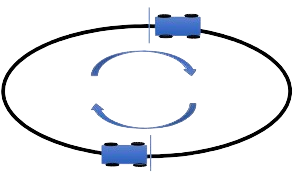
\includegraphics[width=0.50\textwidth]{siguelineas}
	\caption{Circuito para siguelíneas}
	\label{fig:5.1}
\end{figure}

La estrategia más óptima para que PrimeBot pueda realizar esta prueba de forma eficiente es implementando un algoritmo PID (Proporcional, Integral y Derivativo).

\textbf{Algoritmo PID}
 
 El algoritmo PID es un tipo de controlador muy utilizado en sistemas de control. Su objetivo es minimizar la diferencia (el error) entre un valor deseado y el valor real obtenido.
 En nuestro contexto, el valor deseado es que la línea negra esté siempre situada en el centro de los sensores de línea pues en esa posición el error será 0.
 
 Este algoritmo está formado por tres partes:
 \begin{itemize}
\tightlist
\item
  \textbf{Proporcional:} Produce una salida proporcional al error actual, si el error es grande, la salida también lo será.
\item
  \textbf{Integral:} considera la suma acumulada de errores pasados y ayuda a eliminar el error residual que puede persistir si solo se usa la parte proporcional.
\item
  \textbf{Derivativo:} se basa en la tasa de cambio del error, proporciona una predicción de la tendencia del error suavizando la salida.
\end{itemize}

El control PID comienza en PrimeBot con la lectura que se obtiene de los sensores de línea con los que podemos calcular el error de la posición actual.
Cuando ya tenemos el error de posición, podemos calcular la derivada del error (cambio del error con respecto a la lectura anterior)
En la parte integral realizamos la suma acumulativa del error.

Finalmente con las constantes del algoritmo PID y el resto de parámetros calculados realizamos el ajuste en la velocidad de los motores para poder corregir la posición.

Además de este controlador para el seguimiento de la línea, PrimeBot ofrece dentro del código la función \emph{controlador()} que se ha implementado para poder modificar los parámetros del control PID vía bluetooth a través del puerto serial.

Los parámetros configurables son los siguientes:

\begin{itemize}
\tightlist
\item
  \textbf{P:} Aumentará la variable Kp en 0.1
  \item
  \textbf{p:} Reducirá la variable Kp en 0.1
  \item
  \textbf{I:} Aumentará la variable Ki en 0.01
   \item
  \textbf{i:} Reducirá la variable Ki en 0.01
   \item
  \textbf{D:} Aumentará la variable Kd en 0.1
   \item
  \textbf{d:} Reducirá la variable Kd en 0.1
   \item
  \textbf{V:} Aumentará la variable Kv en 0.01
   \item
  \textbf{v:} Reducirá la variable Ki en 0.01
   \item
  \textbf{B:} Aumentará la variable Velocidad base en 1
   \item
  \textbf{b:} Reducirá la variable Velocidad base en 1
\end{itemize}

\subsubsection{5.3.3 Prueba de resolución de cuadrícula}\label{cuadrícula}

La prueba de la cuadrícula consiste en el recorrido desde un punto de origen o estación de origen a un punto de destino o estación de destino.

\begin{figure}[h]
	\centering
	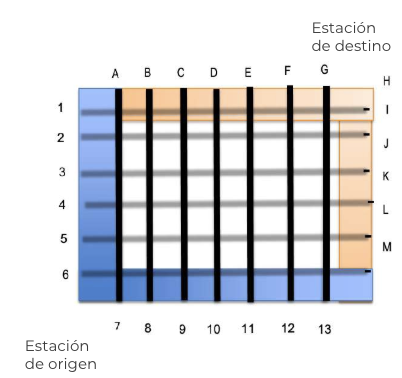
\includegraphics[width=0.50\textwidth]{cuadricula}
	\caption{Cuadrícula ASTI Robotics Challenge}
	\label{fig:5.2}
\end{figure}

El número de estaciones de origen y de destino se conocen de antemano y se numeran con números las estaciones de origen y con letras las estaciones de destino (Figura 5.2).

Para la resolución de esta prueba se requiere de un buen funcionamiento de siguelíneas ya que es la forma en la que el robot va de un punto a otro, siguiendo una línea negra.

Unas peculiaridades de la cuadrícula es que las estaciones de origen y de destino no están conectadas entre sí por tanto no se pueden emplear como puntos intermedios en la ruta calculada sino que solo pueden ser el punto inicial o el final.

Otra peculiaridad es que el usuario puede definir también puntos de la cuadrícula que no están disponibles y que por tanto no se podrán emplear a la hora de calcular el camino más óptimo.

\textbf{Algoritmo A*}

El algoritmo A* es un algoritmo de búsqueda de caminos que busca encontrar la ruta más corta entre dos puntos. 
Combina las estrategias de búsqueda de coste uniforme y búsqueda heurística que permite encontrar soluciones óptimas de forma eficiente.

Este algoritmo es capaz de buscar la ruta más corta desde un nodo inicial (estación de origen) hasta un nodo objetivo (estación de destino).

Para su ejecución se comienza inicializando una lista abierta que contiene los nodos que deben ser evaluados y una lista cerrada que contiene los nodos que ya han sido evaluados.

Cuando el usuario introduce la estación de origen elegida, este punto se añade a la lista abierta como nodo inicial.

Mientras la lista abierta no está vacía, el algoritmo selecciona de forma recurrente el nodo con el menor coste de la lista abierta y lo establece como nodo actual, si este nodo es el nodo objetivo se habrá encontrado una ruta y se puede reconstruir el camino para ejecutarlo después.

Para cada vecino del nodo actual se tiene en cuenta si está o no en la lista cerrada, en caso de estarlo, este nodo se ignorará.
En caso de que no esté en la lista cerrada, se calcula el coste desde el nodo inicial hasta el nodo vecino y si este nodo vecino no está en la lista abierta o el nuevo coste desde el origen es menor que el coste calculado previamente para este vecino se actualizarán los valores de los costes, se establecerá el nodo actual como el padre del vecino y si el vecino no está en la lista abierta, se agregará.

Una vez se encuentra el nodo objetivo, se reconstruye la ruta desde el nodo objetivo hasta el nodo inicial siguiendo los nodos padre.

\subsubsection{5.3.4 Prueba del "laberinto"}\label{laberinto}

En la prueba del laberinto PrimeBot tiene que ir desde la zona de origen hasta el final del laberinto y salir de él (Figura 5.3).
El desarrollo de la prueba tiene que ser totalmente autónomo y evitando tocar las paredes el laberinto.

\begin{figure}[h]
	\centering
	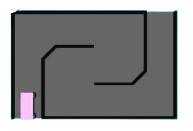
\includegraphics[width=0.50\textwidth]{laberinto}
	\caption{Laberinto ASTI Robotics Challenge}
	\label{fig:5.3}
\end{figure}

Para llevar a cabo esta prueba se utilizan los sensores OPT3101 nombrados anteriormente. 
Esta placa de sensores dispone de 3 canales (TX0,TX1,TX2) con los que podemos detectar objetos a la izquierda del robot, de frente y en el lado derecho proporcionando un ángulo de visión total de 160°.

Para realizar la resolución de los laberintos se ha utilizado la técnica de seguir pared.
El robot seguirá la pared de la derecha o de la izquierda en función de lo que el usuario seleccione vía Bluetooth.

Esta técnica se ha seleccionado ya que la complejidad de los laberintos es baja y no se encuentran laberintos infinitos en los que pueda entrar PrimeBot en bucle.
\newpage
\section{Consideraciones Adicionales}\label{consideraciones}

\textbf{Aspectos que se han tenido en cuenta a la hora de la programación}

\begin{itemize}
\tightlist
\item
  \textbf{Gestión de memoria:} Arduino nano tiene unas capacidades limitadas y con este tipo de algoritmos puede verse limitado en cuanto a memoria a la hora de calcular las rutas, debido a ello se han incorporado funciones que hacen liberación de nodos ya evaluados para reducir el consumo de memoria.
\item
  \textbf{Puntos no disponibles:} se ha tenido en cuenta que los cuatro puntos correspondientes a las esquinas de la cuadrícula no están disponibles y también que cuando el usuario selecciona una estación de origen y una de destino, el resto de estaciones se añaden a la lista de puntos no disponibles para evitar su uso en el cálculo de la ruta.
\end{itemize}


\textbf{Funciones adicionales implementadas en PrimeBot: }
\begin{itemize}
\tightlist
\item
    \textbf{Representación gráfica:} a través del Bluetooth y el monitor Serial, PrimeBot imprime el recorrido que va a realizar para una estación de origen y de destino dadas.
\item
    \textbf{Conectividad Bluetooth:} con la conectividad inalámbrica se pueden indicar las estaciones de origen y de destino, PrimeBot pedirá estos parámetros de forma cíclica para realizar un mayor número de recorridos.
  \item
    \textbf{Caminos alternativos:} además de indicar vía bluetooth las estaciones de origen y destino del recorrido, se pueden indicar puntos de la cuadrícula que estén bloqueados para que a la hora de calcular la ruta se utilicen caminos alternativos.
\end{itemize}

\newpage
\section{Desarrollo web}\label{web}

El objetivo de la web es complementar la información del proyecto PrimeBot y disponer de un lugar donde esté toda la información disponible y las características principales del proyecto de una forma rápida y visual.

Para desarrollar esta web se ha utilizado un dominio personal en el que no se ha utilizado ningún gestor de contenidos.

Toda la programación se ha realizado con HTML5 + CSS + JavaScript.

Además se añaden documentos gráficos como vídeos de la realización de diferentes pruebas.
\begin{figure}[h]
	\centering
	\includegraphics[width=1\textwidth]{CapturaWeb}
	\caption{Web del proyecto}
	\label{fig:5.5}
\end{figure}